\documentclass[a4paper,12pt]{report}
\usepackage{graphicx}
\usepackage[brazil]{babel}
\usepackage{amsmath,amsfonts}
\usepackage[utf8]{inputenc}
\usepackage{listings}

% Pacotes para tabelas
\usepackage{array,color,colortbl}
\newcommand{\mc}[3]{\multicolumn{#1}{#2}{#3}}
\definecolor{tcA}{rgb}{0.625,0.625,0.6406}

%Config do pacote listings
%usado para incluir codigo fonte
\lstset{numbers=left,
stepnumber=5,
firstnumber=1,
numberstyle=\tiny,
extendedchars=true,
breaklines=true,
frame=tb,
basicstyle=\footnotesize,
stringstyle=\ttfamily,
tabsize=3,
showstringspaces=false
}

% Espa�amento de caracteres as margens
\setlength{\textwidth}{16 cm}
\setlength{\textheight}{22 cm}

\evensidemargin 0 cm
\oddsidemargin  0 cm
\topmargin      0 cm

\usepackage{indentfirst}

% ========= Estilos dos capitulos =============
	\makeatletter
	\def\thickhrulefill{\leavevmode \leaders \hrule height 1ex \kern \z@}
	\def\@makechapterhead#1{%
		\reset@font
		\vspace*{-3.50cm}
		\hspace*{-.1cm}
		\noindent

		\begin{center}
		\begin{tabular}{cc}
			\mc{1}{>{\columncolor{tcA}}c}{\color{white}\scshape \strut \Large \bf{Parte}} &
			\mc{1}{>{\columncolor{black}}c}{\color{white} \LARGE \bfseries \strut \thechapter }\\
                       % \mc{1}{>{\columncolor{tcA}}c}{\color{white}\scshape \strut \LARGE \  } \\
		\end{tabular}
		\end{center}

		\noindent
\includegraphics[width=10.5cm ,height=.15cm ]{Figuras/b.jpg}

		\begin{center}
			\vspace{-.70cm} \Huge \bfseries #1
		\end{center}

		\vspace{-.60cm}
		\hspace{4.310cm}
		
\includegraphics[width=10.5cm ,height=.15cm]{Figuras/ib.jpg}
		\vspace*{.0cm}
	}
	\def\@makeschapterhead#1{%
		\reset@font
		\vspace*{-3.00cm}
		\hspace{-.9cm}
		\noindent
		
\includegraphics[width=10.5cm ,height=.15cm]{Figuras/b.jpg}

		\begin{center}
			\vspace{-.70cm} \Huge \bfseries #1
		\end{center}

\vspace{-.60cm}
		\hspace{4.310cm}
		
\includegraphics[width=10.5cm ,height=.15cm]{Figuras/ib.jpg}
		\vspace*{.0cm}

	}
%=========== Estilo das se��es ===================

\makeatletter
\def\section{\@ifstar\unnumberedsection\numberedsection}
\def\numberedsection{\@ifnextchar[%]
  \numberedsectionwithtwoarguments\numberedsectionwithoneargument}
\def\unnumberedsection{\@ifnextchar[%]
  \unnumberedsectionwithtwoarguments\unnumberedsectionwithoneargument}
\def\numberedsectionwithoneargument#1{\numberedsectionwithtwoarguments[#1]{#1}}
\def\unnumberedsectionwithoneargument#1{\unnumberedsectionwithtwoarguments[#1]{#1}}
\def\numberedsectionwithtwoarguments[#1]#2{%
  \ifhmode\par\fi
  \removelastskip
  \vskip 5ex\goodbreak
  \refstepcounter{section}%
  \hbox to \hsize{\vbox{%
      \noindent
      \leavevmode
      \begingroup
      \Large\bfseries
      \noindent 
\includegraphics[width=10.5cm ,height=.15cm]{Figuras/b.jpg}
      \vskip -3.95ex
      \noindent\thesection\
      #2\par \endgroup

      }}\nobreak
  \vskip 2ex\nobreak
  \addcontentsline{toc}{section}{%
    \protect\numberline{\thesection}%
    #1}%
  }
\def\unnumberedsectionwithtwoarguments[#1]#2{%
   \ifhmode\par\fi
  \removelastskip
  \vskip 5ex\goodbreak
  %\refstepcounter{section}%
  \hbox to \hsize{\vbox{%
      \noindent
      \leavevmode
      \begingroup
      \Large\bfseries
      \noindent 
\includegraphics[width=10.5cm ,height=.15cm]{Figuras/b.jpg}
      \vskip -3.95ex
      %\noindent \  \thesection\
      \noindent #2\par \endgroup

      }}\nobreak
  \vskip 2ex\nobreak
    %\addcontentsline{toc}{section}{%
    %\protect\numberline{\thesection}%
    %#1}%
}
\makeatother

%========= Estilo subsection ====================
\makeatletter
\def\subsubsection*{\@ifstar\unnumberedsubsection\numberedsubsection}
\def\numberedsubsection{\@ifnextchar[%]
  \numberedsubsectionwithtwoarguments\numberedsubsectionwithoneargument}
\def\unnumberedsubsection{\@ifnextchar[%]
  \unnumberedsubsectionwithtwoarguments\unnumberedsubsectionwithoneargument}
\def\numberedsubsectionwithoneargument#1{\numberedsubsectionwithtwoarguments[#1]
{#1}}
\def\unnumberedsubsectionwithoneargument#1{\unnumberedsubsectionwithtwoarguments
[#1]{#1}}
\def\numberedsubsectionwithtwoarguments[#1]#2{%
  \ifhmode\par\fi
  \removelastskip
  \vskip 5ex\goodbreak
  \refstepcounter{subsection}%
  \hbox to \hsize{\vbox{
      \noindent
      \leavevmode
      \begingroup
      \bfseries
      \noindent \thesubsection\ %
      #2\par \endgroup
      \vskip -1.85ex \noindent 
\includegraphics[width=7cm,height=.15cm
]{Figuras/b.jpg}


      }}\nobreak
  \vskip 2ex\nobreak
  \addcontentsline{toc}{subsection}{
    \protect\numberline{\thesubsection}%
    #1}%
  }
\def\unnumberedsubsectionwithtwoarguments[#1]#2{%
   \ifhmode\par\fi
  \removelastskip
  \vskip 5ex\goodbreak
  %\refstepcounter{subsection}%
  \hbox to \hsize{\vbox{
      \noindent
      \leavevmode
      \begingroup
      \bfseries
      \noindent %\thesubsection\ %
      #2\par \endgroup
      \vskip -1.85ex \noindent 
\includegraphics[width=7cm,height=.15cm
]{Figuras/b.jpg}


      }}\nobreak
  \vskip 2ex\nobreak
  %\addcontentsline{toc}{subsection}{
    %\protect\numberline{\thesubsection}%
    %#1}%

  }
\makeatother

\begin{document}

% ================ Come�o da capa ===================
	\begin{titlepage}

		\begin{center}
			\begin{figure}[htb]
			\begin{center}

\noindent\hspace*{-.12cm}
\includegraphics[scale=.6]{Figuras/dcc.jpg}
				\noindent\hspace*{12.3 cm}
\includegraphics[scale
= 0.6]{Figuras/icex.jpg}
			\end{center}
			\end{figure}

		\vspace*{-2.45cm}

		\large{
			\hspace{-.5cm}UNIVERSIDADE FEDERAL DE MINAS GERAIS -
UFMG\\
			\hspace{-.5cm}INSTITUTO DE CIÊNCIAS EXATAS - ICEx\\
			\hspace{-1cm}DEPARTAMENTO DE CIÊNCIA DA COMPUTAÇÃO \\

			\hspace{-.5cm}TÓPICOS EM DEPENDABILIDADE
		}

		\vspace{4cm}

		\begin{figure}[htb]
			\begin{center}


\includegraphics[scale=0.5]{Figuras/UFMGdagua.jpg}
			\end{center}
		\end{figure}

		\vspace*{-5.15cm}
		\LARGE{\textbf{Especificação}}
		\par\medskip\normalfont\Large\textbf{Etapa 01
		\linebreak}

		\begin{flushleft}
		\vspace{3cm}
		\large{\hfill Daniel Galinkin da Gama Cerqueira}\\
                \large{\hfill dggc@dcc.ufmg.br}\\
		\large{\hfill Luiz Felipe Mendes}\\
                \large{\hfill lfmendes@dcc.ufmg.br}\\
		\large{\hfill Victor Josué de C. dos G. di Salles e Ferreira}\\
                \large{\hfill josue@dcc.ufmg.br}\\
		\end{flushleft}

		\vspace{3cm}
		\today

	\end{center}
	\end{titlepage}
% =========== fim da capa ==================

% ===== Configuração do texto ==============
	\baselineskip 0.6cm
	\setlength{\parindent}{1.0cm}
	\medskip
	\tableofcontents

% ========== Início da documentação ==========


\section{Descrição do sistema}
Buzzmap é uma ferramenta que propicia o serviço de inteligência
competitiva em redes sociais, criada com o intuito de facilitar e
auxiliar o monitoramento de marcas e opiniões na internet, vigiando
canais de comunicação como Twitter e Youtube.

Esta ferramenta é utilizada basicamente por dois tipos de usuários:
\begin{description}
    \item[Analista] Este usuário da ferramenta a utiliza com o intuito
    de analisar o conteúdo coletado dos canais de comunicação, e gerar
    relatórios e gráficos que sintetizam informações valiosas a
    respeito de um certo assunto.

    \item[Cliente] Este usuário da ferramenta a utiliza com o intuito
    de visualizar os relatórios gerados pelos analistas a respeito de
    determinado assunto.
\end{description}

O sistema está em desenvolvimento e em uso há aproximadamente 10 meses,
sendo que o uso provê feedback e sugestões para a equipe
desenvolvimento.

\chapter{Definição dos requisitos, atores e casos de uso}

\section{Atores}
\begin{description}
    \item[Desenvolvedor] Desenvolvedores do sistema em si. Esse
    projeto esta em constante contrução e aperfeiçoamento, logo o
    desenvolvedor.

    \item[Administrador] É um analista com maiores permissões. Além de
    analisar, administra o projeto e os analistas.

    \item[Analista] Usuário principal do sistema, faz análises de
    conteúdo buscado na internet.

    \item[Cliente] Empresa ou pessoa que contratou o serviço
    oferecido.
\end{description}


\section{Requisitos}
\begin{itemize}
    \item A interface gráfica tem que ser acessível via um browser
    pela internet.
    \item Dado um conjunto de palavras chaves o sistema tem de ter a
    capacidade de coletar conteúdo em diversos canais(orkut, flickr,
            blog, twitter).
    \item O sistema deve ter uma interface gráfica que mostra o
    conteudo coletado.
    \item O sistema deve ter uma interface que dá capacidade de se
    analisar o conteúdo coletado.
    \item O sistema deve ser capaz de gerar gráficos sobre a análise
    feita.
\end{itemize}

\section{Requisitos de Dependabilidade}
\begin{description}
    \item[Disponibilidade do servidor] O sistema tem que ficar no ar
    durante pelo menos 90\% do tempo durante os horários de análise -
    8:00 as 20:00.
    \item[Safety] O sistema deve fazer um backup do banco de dados de
    12 em 12 horas.
    \item[Security] O sistema deve manter dados de usuários(login e
            senhas) protegidos.
    \item[Security] O sistema deve ter uma divisão de privilégios,
    sendo que algumas informações só podem ser vistas por certos
    usuários.
\end{description}
 


\chapter{Casos de Uso}

\begin{itemize}
    \item Usuário $->$ loga no sistema

Todo usuário, deve poder logar na ferramenta através de seu usuário e senha.



    \item Analista $->$ Loga no sistema $->$ Analise um projeto

O analista, entra no sistema e após escolher o projeto e o
canal(orkut, youtube...) faz a análise  de conteúdo e salva essa
análise no banco de dados.


\item Analista $->$ Loga no Sistema $->$ Visualiza Gráficos

O analista loga no sistema, escolhe um projeto e visualiza os gráficos do conteúdo.



\item Administrador $->$ Loga no Sistema $->$ Cria um projeto 

Administrador loga no sistema, e cria um projeto, com data inicial e final e palavras chaves.


\item Administrador $->$ Loga no Sistema $->$ Adiciona analista

Administrador loga no sistema, adiciona um analista e o associa a um projeto.



\item Adminstrador $->$ Loga no Sistema $->$ Cria relatório

Administrador loga no sistema, entra num projeto e cria um relatório e envia ao cliente.



\item Cliente $->$ Loga no sistema $->$ Visualiza informações provida pelo administrador sobre um determinado projeto

Cliente loga no sistema, visualiza relatório provido pelo administrador

\end{itemize}

\section{Casos de uso}

\begin{figure}[hb]
    \begin{center}
        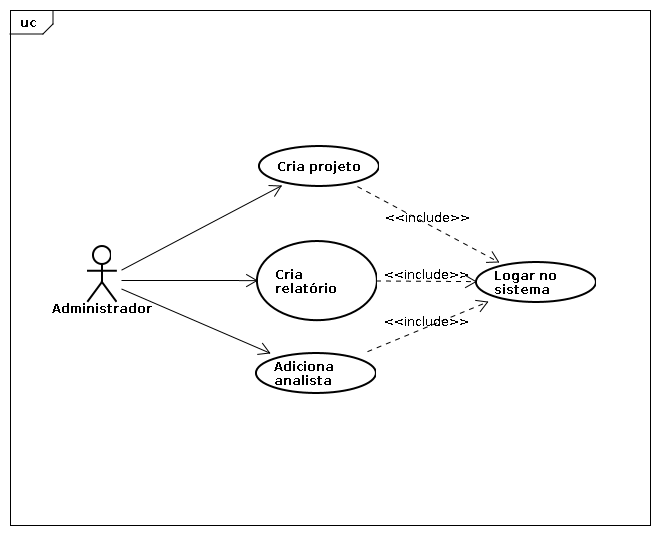
\includegraphics[scale=0.5]{img/caso-uso-administrador.png}
        \caption{Casos de uso do administrador}
        \label{fig:caso-uso-administrador}
    \end{center}
\end{figure}

\begin{figure}[hb]
    \begin{center}
        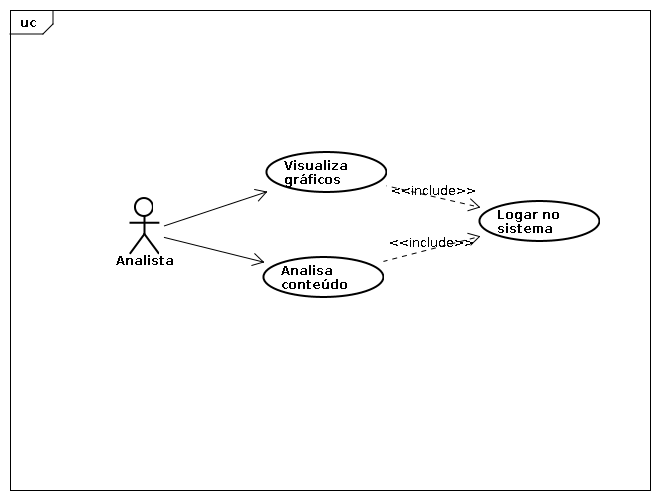
\includegraphics[scale=0.5]{img/caso-uso-analista.png}
        \caption{Casos de uso do analista}
        \label{fig:caso-uso-analista}
    \end{center}
\end{figure}

\begin{figure}[hb]
    \begin{center}
        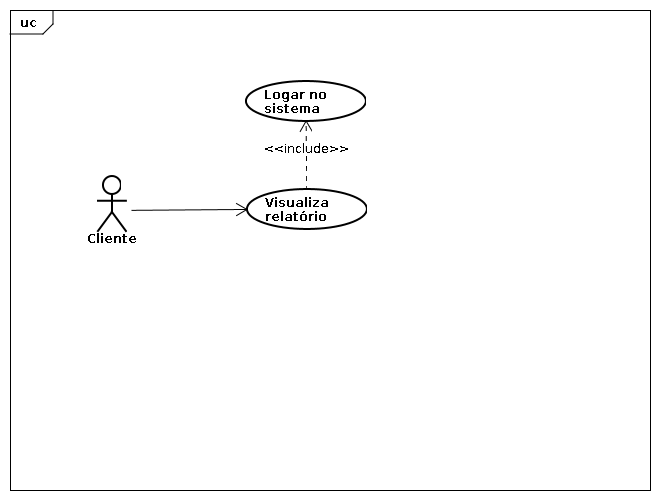
\includegraphics[scale=0.5]{img/caso-uso-cliente.png}
        \caption{Casos de uso do cliente}
        \label{fig:caso-uso-cliente}
    \end{center}
\end{figure}

\section{Especificação UML do Diagrama de Classes do Sistema}

Essa parte do trabalho, que deveria especificar os atributos de cada classe,
assim como as associações entre as classes não pode ser realizada, pois a
ferramenta está atrelada a uma cláusula de sigilo de informações. Por isso,
não podemos divulgar a estrutura das classes com a qual a BuzzMap foi
desenvolvida.


\section{Diagramas de atividades}

\begin{figure}[hb]
    \begin{center}
        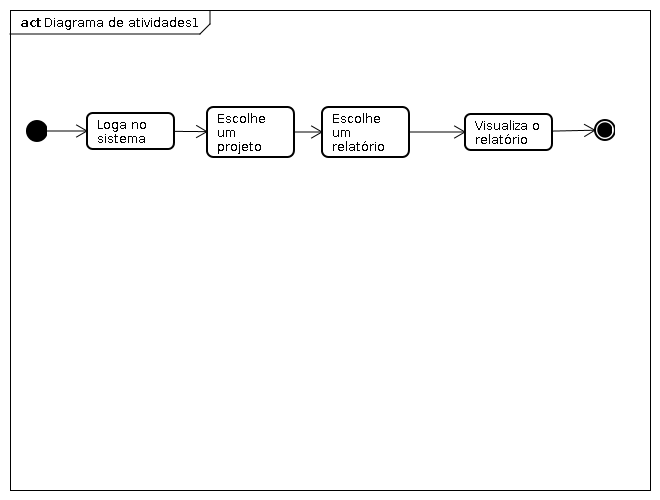
\includegraphics[scale=0.5]{img/atividade1.png}
        \caption{Diagrama de atividades para o caso de uso em que o
            cliente visualiza um relatório.}
        \label{fig:atividade-visualiza}
    \end{center}
\end{figure}

\begin{figure}[hb]
    \begin{center}
        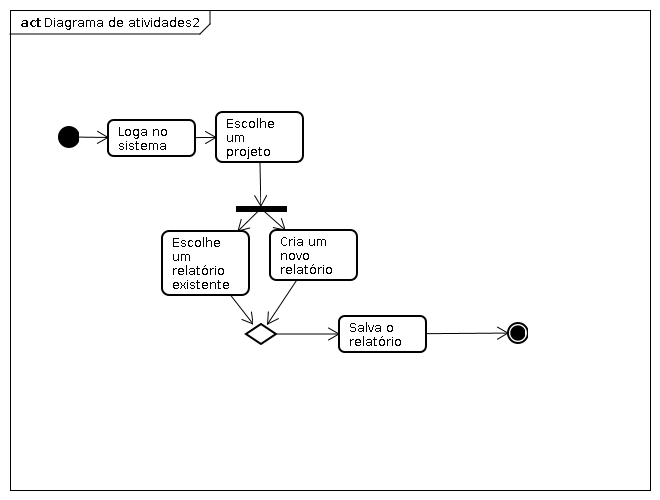
\includegraphics[scale=0.5]{img/atividade2.png}
        \caption{Diagrama de atividades para o caso de uso em que um
            analista gera um relatório.}
        \label{fig:atividade-analisa}
    \end{center}
\end{figure}

\begin{figure}[hb]
    \begin{center}
        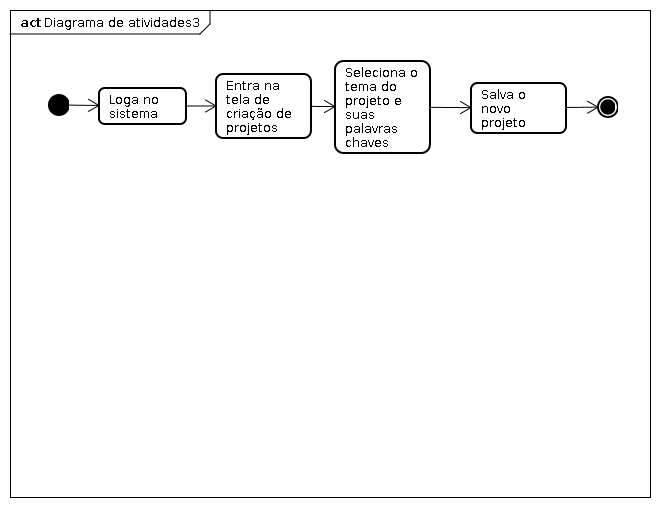
\includegraphics[scale=0.5]{img/atividade3.png}
        \caption{Diagrama de atividades para o caso de uso em que um
            administrador cria um projeto.}
        \label{fig:atividade-cria}
    \end{center}
\end{figure}

\include{questao6}
\section{Visão Geral da Arquitetura e Componentes}


\subsection{Fase 01}

\begin{figure}[hb]
    \begin{center}
        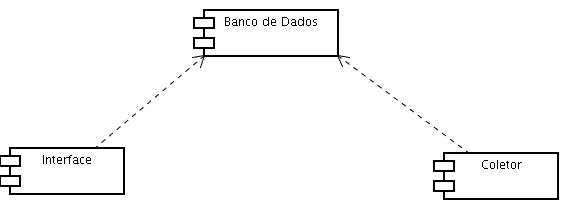
\includegraphics[scale=0.5]{img/conceitual}
        \caption{Arquitetura conceitual geral do sistema}
        \label{fig:arquitetura-conceitual}
    \end{center}
\end{figure}

\subsection{Fase 02}

\begin{figure}[hb]
    \begin{center}
        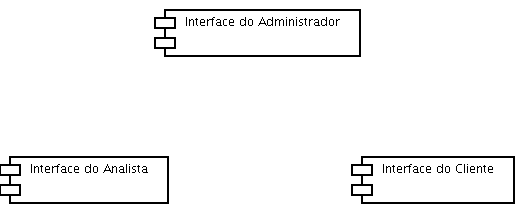
\includegraphics[scale=0.5]{img/interface}
        \caption{Arquitetura dos subsistemas da interface}
        \label{fig:arquitetura-interface}
    \end{center}
\end{figure}

\begin{figure}[hb]
    \begin{center}
        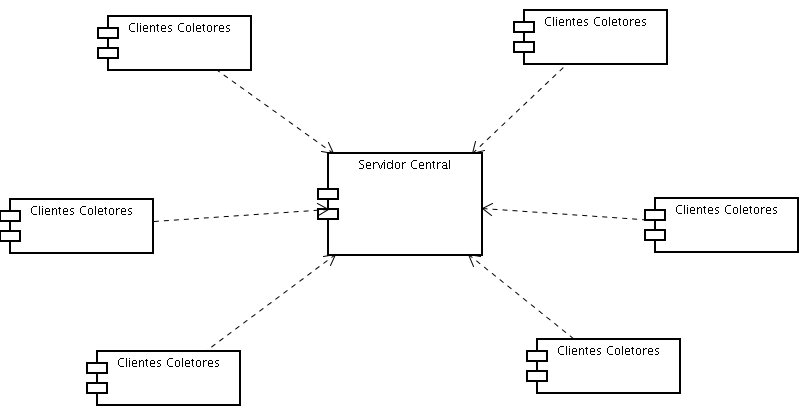
\includegraphics[scale=0.5]{img/coletor}
        \caption{Arquitetura dos subsistemas do coletor}
        \label{fig:arquitetura-coletor}
    \end{center}
\end{figure}

\subsection{Fase 03}

\begin{figure}[hb]
    \begin{center}
        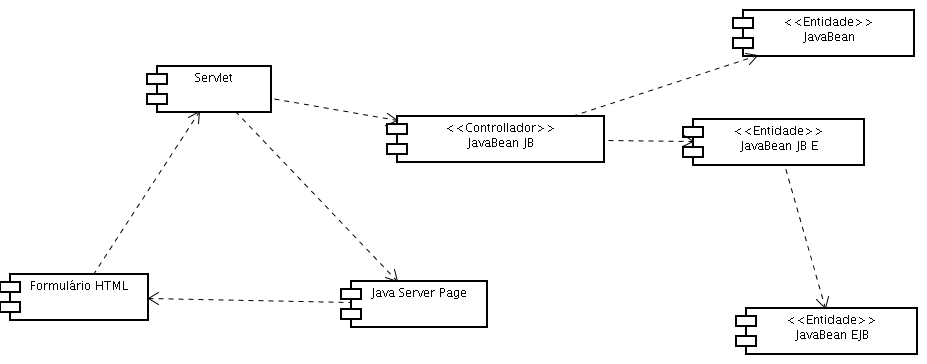
\includegraphics[scale=0.5]{img/jsp}
        \caption{Visão de camadas da implantação JSP}
        \label{fig:}
    \end{center}
\end{figure}


\section{Conclusão}

A realização deste trabalho se mostrou de suma importância, para o
aprofundamento nos conceitos de dependabilidade, pois permitiu a visualização
da ferramenta por diversos aspectos como: disponibilidade(Availability); confiabilidade(Reliability);
segurança(Safety) e proteção (Security). Além disso, a visualização desses aspectos
possibilitou um entendimento ainda maior da Buzzmap e dos
componentes de sua estrutura.

Outro aspecto importante, proporcionado por esse trabalho, foi o conhecimento
construído em relação a dependência dos componentes do sistema e os impactos
que cada um deles possui na ferramenta como um todo. Esse conhecimento foi
adquirido por meio da análise de sensibilidade realizada, que possibilitou
observar a influência isolada desses componentes. 

A maior dificuldade de todo projeto, entretanto, esteve sempre relacionada à
cláusula de privacidade presente no contrato da ferramenta Buzzmap, que
impossibilitou uma exibição de dados mais sensíveis da mesma. Desse modo, ao
contrário do que ocorreu com outros grupos, apesar de possuírmos uma boa gama
de informações sobre o sistema, não foi possível, por exemplo, exibir aspectos
como o diagrama de classes completo da ferramenta.

Enfim, o trabalho proporcionou diversos pontos positivos para todos os membros
do grupo, pois contribuiu para um maior conhecimento da ferramenta e abriu
nossas mentes para futuras melhorias e novos caminhos.


\nocite{wiki:UML, wiki:AD, wiki:UC, ian}
\bibliographystyle{plain}
\bibliography{dependabilidade}

\end{document}

